
\section{Line}
\label{section: line}

グラフがLineの場合,
グラフの全体(頂点と辺)をすべて実直線上におくことができる.
以降,頂点の名前$v_1, v_2, \ldots, v_n$はその位置を表す実数値も表すことにする.

まず,Lineの場合における順序保存運行という特別な運行を定義する.
運行$A$が順序保存であるとは,
$A$が定める巡査の位置$a_1, a_2, \ldots, a_m$が,
任意の時刻$t \in \Rset$において
$a_1(t) \leq a_2(t) \leq \cdots \leq a_m(t)$を満すことである.

Line上の任意の運行$A$は,$A$と同じ数の巡査でかつ警邏する点集合を保ったまま,
順序保存運行$A'$に以下のように変換することができる.
%
まず,$A$が定める各巡査の運行を$a_1, a_2, \ldots, a_m$とする.
これに対し,
$a'_i (i \in \mathset{1, \ldots, m})$を
各時刻$t \in \Rset$において$a' _i(t)$が
$a_1(t), a_2(t), \ldots, a_m(t)$のうち$i$番目に小さいものとなるように定める.
すると,各$a' _i$は運行となっており,
$A' = (a' _i)_{ i \in \mathset{1,\ldots, m} }$とすると
$A'$と$A$の運行の軌跡の集合は等しい
(すなわち,任意の時刻$t \in \Rset$において
$\mathset{a_1(t), \ldots, a_m(t)} = \mathset{a'_1(t), \ldots, a'_m(t)}$)
ので,
$A$で警邏していた点集合を$A'$も警邏している.
これにより順序保存運行$A'$が得られる.
%
順序保存運行$A'$は$A$において巡査がすれ違う時に代わりに
互いの動きを交換することにより順序を保ったものとみなすことができる.

以上から,
巡査$m$人により警邏可能な任意の頂点集合$W$は,
巡査$m$人による或る順序保存運行$A'$によって警邏されることが分かる.




%%%%% section 2.1 %%%%%

\subsection{全点の{\idletime}が等しい場合}
\label{subsec:LineUnaryTimelimit}




本節では次のことを示す.

\begin{theo}
  \label{theo:LineEqualTimelimit}
  グラフの形状がLineで全点の{\idletime}が等しい場合,
  {\patrolling}は多項式時間で解くことができる.
\end{theo}

この問題は,~~な場合については Collinsら~\ref{}の問題の特殊な場合として既に示されているが,
ここでは全点の{\idletime}が等しいという条件のみでも成り立つことを示す.


以降では,
グラフの形状がLineで全点の{\idletime}が等しい場合,
警邏可能な頂点集合のうち利得の和が最大となるものは
次に定義する個別往復運行という運行によって警邏可能であるということを示す.
Lineで全点の{\idletime}が等しい場合に用いることができる
個別往復運行という戦略では
巡査の協力が不要になるため(補題\ref{lemm:LineEqualTimelimitIndependentInterval}),
全点の{\idletime}が等しいという条件が問題を簡単にしているといえる.


\begin{defi}
  $V$を頂点集合,$Q$を各頂点の{\idletime}とする.
  % $m$人の巡査による運行であって,
  % 各巡査が$V$のいずれかの頂点を左端とする長さ$Q/2$の区間を往復する運行を
  % $m$人の巡査による$V$上の個別往復運行と呼ぶ.
  各巡査が$V$のいずれかの頂点を左端とする長さ$Q/2$の区間を往復する運行を個別往復運行と呼ぶ.
  $m$人の巡査による運行$A$において各巡査が個別往復運行をしているとき,
  $A$を単に$m$人の巡査による個別往復運行と呼ぶ.
\end{defi}



まず次の補題を示す.

\begin{lemm}
  \label{lemm:RangeOfPatrollerOnLine}
  頂点$v_i$がある1人の巡査$s$により単独警備されているとき,
  {\idletime}を$q_i$として,
  $s$は常に区間$[v_i - q_i/2, v_i + q_i/2]$にいる.
\end{lemm}

\begin{proof}[証明]
  \newcommand{\vout}{v_{\mathrm{out}}}
  この区間にない或る座標$\vout \notin [v_i - q_i/2, v_i + q_i/2]$を$s$が
  時刻$t_0$に訪問するとする.
  $\vout$と$v_i$の間の移動には
  少くとも時間$\lvert v_i - \vout \rvert > q _i / 2$を要するから,
  $s$は区間$[t_0 - q _i / 2, t_0 + q _i / 2]$に属する時刻に$v_i$を訪問できない.
  この区間の長さは$
    q_i
  $であるので,$s$が$v _i$を単独警備していることに反する.
\end{proof}



これにより次の補題が成り立つ.


\begin{lemm}
 \label{lemm:LineEqualTimelimitIndependentInterval}
  グラフの形状がLineで,頂点の{\idletime}がすべて$Q$であるとする.
  頂点集合$W$が$m$人の巡査により警邏可能であるとする.
  このとき,
  $W$を警邏する$m$人の巡査による個別往復運行が存在する.
\end{lemm}


\begin{proof}[証明]

  \newcommand{\leftmostpoint}{b}  % v以外の記号
  \newcommand{\newpatroller}{l}
  \newcommand{\leftmostpatroller}{a_1}

  巡査数$m$に関する帰納法で示す.
  $m = 0$のときは明らかなので,以下$m > 0$とする.

  $W$は$m$人の巡査により警邏可能であるので,2章始めの議論により$W$を警邏する$m$人の巡査による順序保存運行が存在する.
  このような運行を任意に一つ選び
  $A = (a _i) _{i \in \{1, \ldots, m\}}$
  とする.

  $W$の点のうち最も左にあるものを$\leftmostpoint$とする.
  まず,各巡査は
  $\leftmostpoint$より左に存在する時間
  $\leftmostpoint$で停止するように変換する.
  このようにしても$W$は警邏されたままであり,
  また,これによりすべての巡査は
  $[\leftmostpoint, +\infty)$に存在することになる.

  ここで,最も左の巡査$\leftmostpatroller$に注目する.
  $\leftmostpoint$が$A$により訪問されるすべての時刻に
  $\leftmostpatroller$は$\leftmostpoint$を訪問しているので,
  $\leftmostpoint$は$\leftmostpatroller$により単独警備されている.
  %
  すると,
  補題\ref{lemm:RangeOfPatrollerOnLine}より,
  任意の時刻$t \in \Rset$に対し
  $\leftmostpatroller(t) \leq \leftmostpoint + Q/2$
  であるが,
  %
  一方,$\leftmostpatroller$は区間$[b, b + Q/2]$を速さ$1$で往復することで
  この区間に含まれるすべての頂点を警備することができる.
  実際,$\leftmostpatroller$がこのような往復をするとき
  $\leftmostpoint \leq x \leq \leftmostpoint + Q/2$
  である位置$x$に存在する時刻の間隔の最大値は
  \[
    \max( 2(x - \leftmostpoint), 2(\leftmostpoint + Q/2 - x) )
    \leq 2(\leftmostpoint + Q/2 - \leftmostpoint) = Q
  \]
  より,$[\leftmostpoint, \leftmostpoint + Q/2]$に含まれるどの頂点も
  {\idletime}を超えずに訪問できていることが分かる.
  これにより$\leftmostpatroller$の運行は個別往復運行となる.
  %
  一方,$W^- := \mathsetmid{ v \in W }{ \leftmostpoint + Q/2 < v }$は$\leftmostpatroller$以外の$m - 1$人の巡査により警備されているので,帰納法の仮定から
  残る$m - 1$人の巡査も個別往復運行に変換することができる.
  以上により$W$を警邏する$m$人の巡査による個別往復運行が得られた.
\end{proof}


補題\ref{lemm:LineEqualTimelimitIndependentInterval}により,
個別往復運行を行う場合のみを考えればよいため,
$m$人の巡査がそれぞれ担当する$m$個の区間を求めればよい.
以下のアルゴリズムにより利得の和が最大となる$m$個の区間を求めることができる.

初めにLine上の頂点をソートしておき,左側から順に$v_1,v_2,\ldots,v_n$とする.
頂点$v_i$を左端とする区間を$I_i := [v_i, v_i + Q/2]$と書く.

まず,
$n$個の区間$I_i (i = 1,2,\ldots, n)$について
各区間に含まれる点から得られる利得の合計$P_i$を求める.
$P_i$は$v_1,v_2,\ldots,v_n$がソートしてあるので$O(n)$で求めることができる.

あとは$m$個($m$は巡査の人数)の区間を選び利得の合計を最大化すればよいが,
以下の漸化式\ref{eq:LineWISPDP}に従う動的計画法で
$O(mn)$で
最大の利得を得られる$m$個の区間を選択できる.
$OPT(i,j)$は,区間$I_1, \ldots, I_j$から最大$i$個の区間を選ぶときの
利得の合計の最大値を表す.
$OPT(m,n)$が求めたい利得の最大値となる.
\begin{align}
  \label{eq:LineWISPDP}
  OPT(i,j) = 
  \begin{cases}
    0 & \text{$i = 0$または$j = 0$のとき} \\
    \max \{
      OPT(i, j - 1), 
      P_j + OPT(i - 1, j - 1)
    \}
    & \text{それ以外の場合}
  \end{cases}
\end{align}

最後に,$OPT(m,n)$において選ばれた区間をトレースバックして求め,
この区間に含まれる頂点全体を出力して終了する.

このアルゴリズムの計算量は最初のソートも含めて全体で
$O(n \log n + nm)$となる.
これで定理\ref{theo:LineEqualTimelimit}が示された.



% Circleについて
この証明では線分に端の頂点が存在することが重要な役割を果たしているため,
閉路の場合にそのまま適用することはできない.


\subsection{{\idletime}が一般の場合}
\label{subsec:LineDifferentTimelimit}

全点の{\idletime}が等しい場合は
どの頂点も複数の巡査の協力で警備する必要がないため単純になっていたが,
{\idletime}が一般の場合は,
頂点を複数の巡査が交代で訪問して警備する必要がある場合が存在する.
%
図\ref{tikz:multiAgentExample2}(左)の例では,
中央の{\idletime}の短い2つの頂点を
2人の巡査が交互に訪問しており,
また,全点の{\idletime}が等しい場合と異なり
各巡査の最適な運行はなんらかの区間の往復であるとは限らないことも分かる.


また,
\red{左から巡査の動きを決定できるのではないか?しかし,…
(許容訪問間隔ぴったりの周期の場合についてのみ反例を作る?}
この例では左の巡査は左端の点を{\idletime}$10$ちょうどごとに訪問しているが,
左端の点の{\idletime}から順に巡査の運行を決定することも難しい次のような例が存在する.
図\ref{tikz:multiAgentExample2}(中央)の例では
{\idletime}$8$の左端の点をあえてより短い$6$ごとに訪問することで全点を警邏できるが,
同じグラフについて,
図\ref{tikz:multiAgentExample2}(右)のように左の巡査が
左端の点の{\idletime}ぎりぎりの時間まで右の方へ動き頂点をなるべく多くの時間訪問して左端へ帰る運行を選ぶと
右の巡査がどのような動き方をしても訪問間隔が{\idletime}を超え警備できない頂点が生まれてしまう.



\begin{figure}[h]
  \centering
  \begin{tabular}{ccc}

  \begin{minipage}{0.32\hsize}
    \centering
    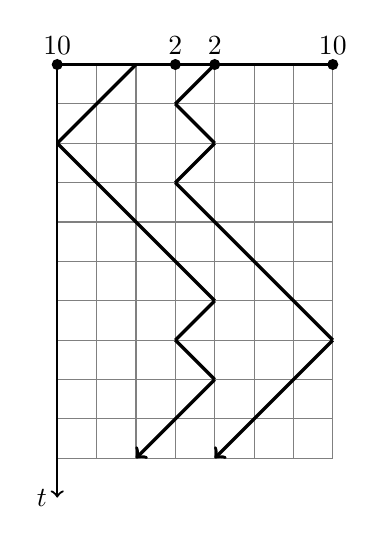
\begin{tikzpicture}
      \draw [help lines,thin,step=5mm] (0,-5.0) grid (3.5,0);
      \draw[thick] (0,0) -- (3.5,0) node [below] {};
      \draw[thick, ->] (0,0) -- (0,-5.5) node [left] {$t$};

      \fill ( 0   , 0) coordinate (c1) circle (2pt) node [above] {10};
      \fill ( 1.5 , 0) coordinate (c2) circle (2pt) node [above] {2};
      \fill ( 2.0 , 0) coordinate (c3) circle (2pt) node [above] {2};
      \fill ( 3.5 , 0) coordinate (c5) circle (2pt) node [above] {10};

      \draw[very thick,- ] ( 1.0, 0  )--(   0,-1.0);
      \draw[very thick,- ] (   0,-1.0)--( 2.0,-3.0);
      \draw[very thick,- ] ( 2.0,-3.0)--( 1.5,-3.5);
      \draw[very thick,- ] ( 1.5,-3.5)--( 2.0,-4.0);
      \draw[very thick,->] ( 2.0,-4.0)--( 1.0,-5.0);

      \draw[very thick,- ] ( 2.0, 0  )--( 1.5,-0.5);
      \draw[very thick,- ] ( 1.5,-0.5)--( 2.0,-1.0);
      \draw[very thick,- ] ( 2.0,-1.0)--( 1.5,-1.5);
      \draw[very thick,- ] ( 1.5,-1.5)--( 3.5,-3.5);
      \draw[very thick,->] ( 3.5,-3.5)--( 2.0,-5.0);
    \end{tikzpicture}
  \end{minipage}

  \begin{minipage}{0.32\hsize}
    \centering
    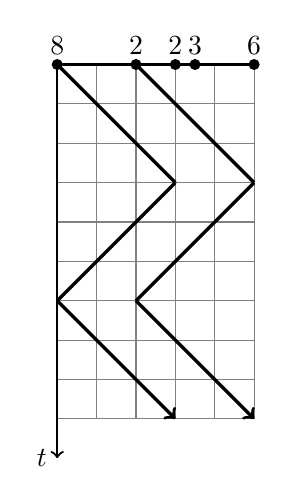
\begin{tikzpicture}
      \draw [help lines,thin,step=5mm] (0,-4.5) grid (2.5,0);
      \draw[thick] (0,0) -- (2.5,0) node [below] {};
      \draw[thick, ->] (0,0) -- (0,-5) node [left] {$t$};

      \fill ( 0   , 0) coordinate (c1) circle (2pt) node [above] {8};
      \fill ( 1   , 0) coordinate (c2) circle (2pt) node [above] {2};
      \fill ( 1.5 , 0) coordinate (c3) circle (2pt) node [above] {2};
      \fill ( 1.75, 0) coordinate (c4) circle (2pt) node [above] {3};
      \fill ( 2.5 , 0) coordinate (c5) circle (2pt) node [above] {6};

      % \draw[very thick,red,<->] (1.75,-0.75)--(1.75,-2.25);

      \draw[very thick,- ] ( 0  , 0  )--( 1.5,-1.5);
      \draw[very thick,- ] ( 1.5,-1.5)--( 0  ,-3  );
      \draw[very thick,->] ( 0  ,-3  )--( 1.5,-4.5);
      \draw[very thick,- ] ( 1  , 0  )--( 2.5,-1.5);
      \draw[very thick,- ] ( 2.5,-1.5)--( 1  ,-3  );
      \draw[very thick,->] ( 1  ,-3  )--( 2.5,-4.5);
    \end{tikzpicture}
  \end{minipage}

  \begin{minipage}{0.32\hsize}
    \centering
    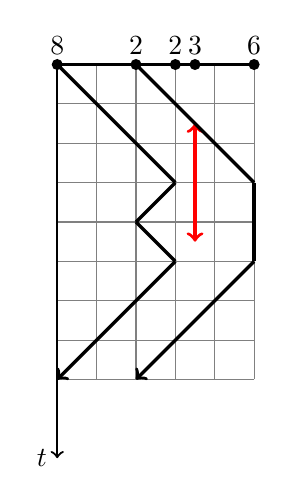
\begin{tikzpicture}
      \draw [help lines,thin,step=5mm] (0,-4) grid (2.5,0);
      \draw[thick] (0,0) -- (2.5,0) node [below] {};
      \draw[thick, ->] (0,0) -- (0,-5) node [left] {$t$};

      \fill ( 0   , 0) coordinate (c1) circle (2pt) node [above] {8};
      \fill ( 1   , 0) coordinate (c2) circle (2pt) node [above] {2};
      \fill ( 1.5 , 0) coordinate (c3) circle (2pt) node [above] {2};
      \fill ( 1.75, 0) coordinate (c4) circle (2pt) node [above] {3};
      \fill ( 2.5 , 0) coordinate (c5) circle (2pt) node [above] {6};

      \draw[very thick,red,<->] (1.75,-0.75)--(1.75,-2.25);

      \draw[very thick,- ] ( 0  , 0  )--( 1.5,-1.5);
      \draw[very thick,- ] ( 1.5,-1.5)--( 1  ,-2  );
      \draw[very thick,- ] ( 1  ,-2  )--( 1.5,-2.5);
      \draw[very thick,->] ( 1.5,-2.5)--( 0  ,-4  );

      \draw[very thick,- ] ( 1  , 0  )--( 2.5,-1.5);
      \draw[very thick,- ] ( 2.5,-1.5)--( 2.5,-2.5);
      \draw[very thick,->] ( 2.5,-2.5)--( 1  ,-4  );
    \end{tikzpicture}
  \end{minipage}

  \end{tabular}
  \caption{巡査の協力が必要な例.
    横軸を頂点の座標,縦軸を時刻として巡査の軌跡を表す.
    点の上の数値は{\idletime}を表す.
    \label{tikz:multiAgentExample2}}
\end{figure}




これらの例は,協力が発生する場合巡査の運行を個別に決定するのは難しいということを示唆している.
しかしながら,この許容訪問間隔が一般の場合でのLine上の協力警邏問題の困難性を示すこともできなかった.

そこで我々は,あえて{\idletime}より短い周期で点を訪問すること許されていたことが
運行の決定を複雑にしていたことを踏まえて,
より自由度の少ない条件として,
ある訪問時刻とその時刻からの厳密な訪問間隔が指定され,
それらの時刻すべてにちょうど訪問しなければならない
という別種の問題(「時刻指定協力警邏問題」と呼ぶことにする)も調べた.
すなわち,警備の条件を次のようにする.

\begin{defi}
  運行$A = (a _i) _{i \in \{1, \ldots, m\}}$が
  点$v \in U$を厳密訪問間隔$(q, r)$で警備するとは,
  任意の時刻$t := q k + r (k \in \Zset)$に対し
  巡査$i$が存在し
  $a _i (t) = v$
  であることをいう.
\end{defi}
%
この「時刻指定協力警邏問題」でかつ全点を警邏可能かを判定する問題であれば,
以降示すように巡査の動きを端から順に個別に決定できることが分かった.


\begin{defi}
  図\ref{tikz:defLR}のように$x$-$t$平面の点$a = (x_a, t_a)$に対して領域$L(a), R(a)$を
  \begin{align*}
    L(a) &:= \mathsetmid{(x, t)}{ x - x_a \leq |t - t_a| } \\
    R(a) &:= \mathsetmid{(x, t)}{ x - x_a >    |t - t_a| }
  \end{align*}
  と定義する.

  訪問しなければならない位置と時刻の組の集合$X$が与えられたとき,
  $\dbigcap_{a \in X} L(a)$の境界線が軌跡であるような運行を
  「最右運行」と定義する.
\end{defi}

\begin{figure}[h]
  \centering
  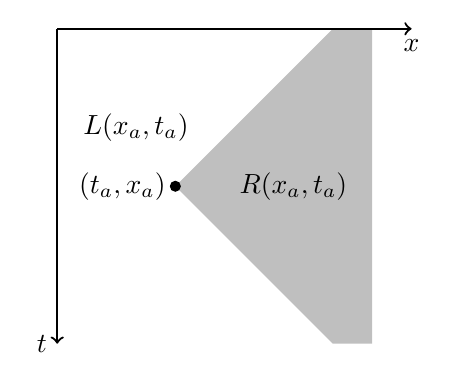
\begin{tikzpicture}
    \fill [fill=lightgray]
      (1.5, -2)--(3.5,0)--(4,0)--(4,-4)--(3.5,-4)--(1.5, -2);

    % \draw [help lines, thin,step=10mm] (0,-5.5) grid (5.5,0);
    \draw[thick, ->] (0,0) -- (4.5, 0) node [below] {$x$};
    \draw[thick, ->] (0,0) -- (0,-4) node [left] {$t$};

    \fill ( 1.5,-2) coordinate (a) circle (2pt) node [left] {$(t_a,x_a)$};

    \node (L) at (1,-1.25) {$L(x_a, t_a)$};
    \node (R) at (3,-2) {$R(x_a, t_a)$};
  \end{tikzpicture}
  \caption{$L(x_a, t_a)$ と $R(x_a, t_a)$ の定義 \label{tikz:defLR}}
\end{figure}

三角形領域$R(x_a, t_a)$は,
時刻$t_a$に$x_a$に存在する巡査が存在し得ない位置と時刻の組の集合のうち
$x_a$より右側の領域を表している($|x - x_a| / |t - t_a| > 1$かつ$x_a < x$).
訪問しなければならない位置と時刻の組の集合$X$に対して,
$\dbigcap_{a \in X} L(a)$は
一番左の巡査の存在可能領域を表す(補題**).



本節で示すのは以下の定理である.
\begin{theo}
  \label{lemm:LineExactFinite}
  グラフの形状がLineのとき,
  時刻指定協力警邏問題は,
  「最右運行」で巡査の運行を左端から順に決定する\red{(←手順が未定義)}ことで
  全点警邏可能か判定できる.
  \red{
    指定時刻が有限個ならその個数の多項式時間で判定できる、とかにする?
    入力が周期と剰余なら$O(*)$で計算できる、とかに?
  }
\end{theo}


\begin{lemm}
  \label{lemm:leftmostAgentExistableTerrain}
  $X$を訪問しなければならない位置と時刻の組の集合とする.
  このとき,
  順序保存運行において一番左の巡査$s$の軌跡は
  $\bigcap_{a \in X} L(a)$に含まれる.
\end{lemm}

\begin{proof}
  巡査$s$の軌跡に$\bigcup_{a \in X} R(a)$の点$b = (x_b, t_b)$が含まれるとすると,
  ある$a = (x_a, t_a) \in X$が存在して$b \in R(a)$となる.
  巡査の速さは1以下なので時刻$t_a$における巡査$s$の位置$x$は
  $|x_b - x| \leq |t_b - t_a|$を満たすが,
  $b \in R(a)$より$x_b - x_a > |t_b - t_a|$なので
  $x_b - x \leq |x_b - x| < x_b - x_a$,
  すなわち$x_a < x$となる.
  $x_a < x$より$x_a$を警備する$s$より左の巡査が必要になり矛盾する.
  よって,$s$の軌跡は$\bigcup_{a \in X} R(a)$の点を含まない.
\end{proof}

これにより次がいえる.

\begin{lemm}
  \label{lemm:LineExactFinite}
  グラフ$G$がLineのときの時刻指定協力警邏問題において,
  $m$人の巡査により$G$を警邏可能であるとき,
  $m$人の巡査による一番左の巡査が最右運行である順序保存運行により$G$を警邏できる.
\end{lemm}

\begin{proof}
  指定時刻の集合を$X$とする.
  $G$は$m$人の巡査により警邏可能であるので,
  2章始めの議論により$G$を警邏する$m$人の巡査による順序保存運行が存在する.
  このような運行を任意に一つ選び$A$とする.
  補題\ref{lemm:leftmostAgentExistableTerrain}より$A$における一番左の巡査$s$の軌跡は
  $\bigcap_{a \in X} L(a)$に含まれる.
  $b(X)$を$\bigcap_{a \in X} L(a)$の境界線とする.\red{(←先に定義しておく)}
  $\bigcap_{a \in X} L(a)$に含まれる$X$の点は$\bigcap_{a \in X} L(a)$の境界線上に存在するので
  $s$の軌跡に含まれる点全体は$b(X)$の部分集合となるが,
  一方,$s$が$b(X)$が軌跡であるような運行を代わりに行うと,
\end{proof}

% 全点を警備する任意の順序保存運行$A$で一番左側を動く巡査$s_1$の軌跡を考える.
% %
% もし$t$-$x$平面上のある点$(t_a,x_a)$から定まる$R(t_a,x_a)$に含まれる点$(t',x')$を
% $s_1$の軌跡が通っているとすると,
% $s_1$は$|x_a - x'| > |t_a - t'|$より時刻$t_a$に座標$x_a$を訪問できないので
% $s_1$が一番左側を動くことから$(t_a,x_a)$が訪問されない点となってしまい矛盾する.
% %
% よって,$A$で一番左側を動く巡査$s_1$の軌跡は$\dbigcap_{a \in X'} L(a)$に含まれる.
% $L(X') := \dbigcap_{a \in X'} L(a)$とする.

% 一方,この領域$L(X')$の境界線は傾き$1$または$-1$の線分のつながったものであるので,
% $s_1$はこの境界線が軌跡となるように動くことができ,
% そのようにすることで$L(X')$に含まれるすべての点を訪問でき
% $A$での$s_1$の動きを改善できる.
% %
% $s_2, s_3, \ldots, s_m$の動き方も$X'$ の残りの点に対して
% $s_1$のときと同様に決めていくことで$A$での動きを改善できる.
